% CREDITS:
% Comprehensive exam template for ECE Ph.D. students at Queen's University. by Jefferson Silveira
\documentclass[a4paper,12pt]{article}
\usepackage[left=30mm,top=30mm,right=30mm,bottom=30mm]{geometry}
\usepackage{etoolbox} %required for cover page
\usepackage{booktabs}
\usepackage[usestackEOL]{stackengine}
\usepackage[T1]{fontenc}
\usepackage[utf8]{inputenc}
\usepackage{bm}
\usepackage{graphicx}
\usepackage{subcaption}
\usepackage{amsmath}
\usepackage{amsfonts}
\usepackage{mathtools}
\usepackage{xcolor}
\usepackage{float}
\usepackage{hyperref}
\usepackage[capitalise]{cleveref}
\usepackage{enumitem,kantlipsum}
\usepackage{amssymb}
\usepackage[square,numbers,sort]{natbib}
\usepackage[ruled,vlined]{algorithm2e}
\usepackage{listings}
\usepackage{minted}
\usemintedstyle{emacs}
% \usepackage[portuguese]{babel} % uncomment for portuguese commands

\renewcommand{\listingscaption}{Algorithm}
\renewcommand{\listoflistingscaption}{List of Algorithms}

\bibliographystyle{unsrtnat}

\hypersetup{
    colorlinks,
    linkcolor={black},
    citecolor={blue!50!black},
    urlcolor={blue!80!black}
}

\linespread{1}

\newtheorem{theorem}{Theorem}[section]
\graphicspath{{figures/}}	

% ------------------- important:

\begin{document}

\pagenumbering{gobble} % remove page numbers (and reset to 1)

% -------------------------------- Front page
% -------------------------------- "Global front stuff" xd
\newcommand{\docenteUM}{Docente 1}
\newcommand{\docenteDOIS}{}
\newcommand{\docenteTRES}{}

\newcommand{\data}{Abril 2022} % CHANGE HERE
\date{Abril 2022} % idk, didnt work xd

\newcommand{\subtitle}{Subtítulo}
\newcommand{\titulo}{Título} % CHANGE HERE
\title{Título}
\newcommand{\departmento}{Departamento de Engenharia Eletrónica e de
Telecomunicações e Computadores}
\newcommand{\curso}{Licenciatura em Engenharia Informática e de Computadores}

% -------------------------------- Front content
\begin{center}\leavevmode
    \normalfont
    
\includegraphics[width=0.75\columnwidth]{img/isel.jpg}
    \vskip 1cm 
    \textsc{\Large \departmento}\\[1 cm]
    {\large \curso}
    \vskip 1cm
    \rule{\linewidth}{0.2 mm}
    {\huge \bfseries \titulo \par}
    \vskip 1cm
    {\Large \bfseries \subtitle \par}
           
    \rule{\linewidth}{0.2 mm}\\[1.5 cm]
     
    \begin{minipage}[t]{0.45\textwidth}
    	\begin{flushleft} \large
    		\emph{Alun@s:}\\
    		A11231 - Nome Aluno 1\\
    		A48121 - Nome Aluno 2\\
    		A39411 - Nome Aluno 3
    	\end{flushleft}
    \end{minipage}
    \begin{minipage}[t]{0.45\textwidth}
        \begin{flushright} \large
        	{\emph{Docentes:}}\\
        	\ifdefempty{\docenteUM}{}{\docenteUM\\}
        	\ifdefempty{\docenteDOIS}{}{\docenteDOIS\\}
        	\ifdefempty{\docenteTRES}{}{\docenteTRES\\}
        \end{flushright}
    \end{minipage}
    \vfill
    {\normalsize \data\par}
\end{center}
\cleardoublepage
\tableofcontents
\newpage
%\listoffigures
%\newpage
%\listoftables
%\newpage
%\listofalgorithms % List of algorithms in pseudocode format
%\newpage
%\listoflistings % List of algorithms in code format
%\newpage

\pagenumbering{arabic} % Arabic page numbers (and reset to 1)

% Sections
\section{Introduction}
\section{Section 1}
\subsection{Subsection 1}
\subsubsection{Subsubsection 1}
You won't find subsubsubsections but you can also add a paragraph
\paragraph{Paragraph} 

if you really need another layer.

But you can also modify the document if you really need more subsections.

\section{Examples} \label{sec:section2}

This is how you reference labels. Section \ref{sec:section2} explains how to reference labels. Section \ref{sec:citing} explains how to cite papers.

\subsection{Citing}\label{sec:citing}
This is one citation \cite{Mabuchi2012}. This is another citation \cite{HAN201687}. You can aggregate citations \cite{Mabuchi2012, HAN201687}.

\subsection{Theorem}
\begin{theorem} \label{theo:theorem1}
This is one way to define a theorem
\end{theorem}

You can also reference the Theorem \ref{theo:theorem1}.

\subsection{Coloring text for revision}
\textcolor{red}{You can color your text in case you want to add comments during the review of your comp I}.

\subsection{Adding images}
This is how you reference an image Figure \ref{fig:example_1}.

\begin{figure}[ht]
    \centering
    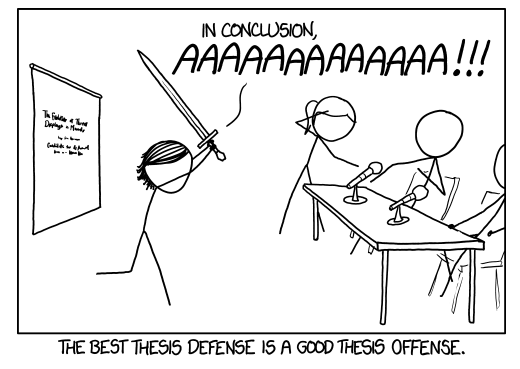
\includegraphics[width = 0.3\linewidth]{img/Thesis_Defence.png}
    \caption{You can cite the source in the caption \cite{xkcd}.}
    \label{fig:example_1}
\end{figure}

This is how you reference a sub-image Figure \ref{fig:a}.

\begin{figure}[ht] 
  \begin{subfigure}[b]{0.5\linewidth}
    \centering
    \includegraphics[width=0.6\linewidth]{example-image-a}
    \caption{Image a} 
    \label{fig:a} 
    \vspace{4ex}
  \end{subfigure}%% 
  \begin{subfigure}[b]{0.5\linewidth}
    \centering
    \includegraphics[width=0.6\linewidth]{example-image-b} 
    \caption{image b} 
    \label{fig:b} 
    \vspace{4ex}
  \end{subfigure} 
  \begin{subfigure}[b]{0.5\linewidth}
    \centering
    \includegraphics[width=0.6\linewidth]{example-image-c} 
    \caption{image c} 
    \label{fig:c} 
  \end{subfigure}%%
  \begin{subfigure}[b]{0.5\linewidth}
    \centering
    \includegraphics[width=0.6\linewidth]{example-image-duck}
    \caption{image d} 
    \label{fig:d} 
  \end{subfigure} 
  \caption{This is how you can create many images at once.}
  \label{fig:example_many_images} 
\end{figure}

\subsection{Adding equations}

Equation \ref{eq:euler} is Euler's favorite equation. Maybe you want to cite as IEEE style? \eqref{eq:euler} shows Euler's favorite equation.

\begin{equation}
\label{eq:euler}
    e^{i\pi} + 1 = 0
\end{equation}

\subsection{Adding tables}

Table \ref{tab:table1} is a simple table.
\begin{table}[H]
  \caption{This is a simple table}
  \label{tab:table1}
  \centering
  \begin{tabular}{lccc}
  \toprule
    Class       &   Feature 1   &   Feature 2   &   Feature 3   \\
    \midrule
    Class 1     &   a   &   a   &   a   \\
    Class 2     &   a   &   a   &   a   \\
    \bottomrule
  \end{tabular}
\end{table}


Table \ref{tab:table2} contains more advanced components.
\begin{table}[H]
  \caption{This is a comprehensive table}
  \label{tab:table2}
  \centering
  \begin{tabular}{lcccc}
  \toprule
  & \multicolumn{2}{c}{CNN} & \multicolumn{2}{c}{CNN+LSTM} \\
  \cmidrule(r){2-3} \cmidrule(r){4-5}
    Difficulty     & Model 1 &  Model 2 & Model 1 & Model 2\\
    \midrule
    Easiest   & \Centerstack{ calm \\ angry \\ neutral}  &   \Centerstack{ angry \\ disgust \\ surprised}   &   \Centerstack{ calm \\ angry \\ neutral} & \Centerstack{ angry \\ fearful \\ calm} \\
    \midrule
    Hardest & \Centerstack{ sad \\ surprised \\ happy}   & \Centerstack{ neutral \\ sad \\ happy/fearful} & \Centerstack{ sad \\ surprised \\ happy/disgust}   &   \Centerstack{ neutral/sad \\ happy \\ disgust } \\
    \bottomrule
  \end{tabular}
\end{table}


\subsection{Lists}
This is an unordered list
\begin{itemize}
    \item Item 1
    \item Item 2
\end{itemize}

This is an ordered nested list
\begin{enumerate}
    \item Item 1
    \begin{enumerate}
        \item Item one
        \item Item two
        \item Item three
    \end{enumerate}
    \item Item 2
\end{enumerate}

\subsection{Algorithms}

Algorithm \ref{alg:algorithm1} shows how to write pseudocode.

\begin{algorithm}
\KwResult{Write here the result }
 initialization\;
 \While{While condition}{
  instructions\;
  \eIf{condition}{
   instructions1\;
   instructions2\;
   }{
   instructions3\;
  }
 }
 \caption{Example of algorithm}
 \label{alg:algorithm1}
\end{algorithm}

You can also import code, if you really need to show the exact code that you used. For example, Algorithm \ref{listing:research} shows how to do research.

\begin{center}
\begin{listing}[H]
\centering

% if you want to use a file to show the whole code
% \inputminted{python}{codes/research.py}

\begin{minted}{c++}
#include <stdio.h>

int main(int argc, char** argv) {
    std::cout << "boas";
    return 0;
}
\end{minted}

\caption{How to do research}
\label{listing:research}
\end{listing}
\end{center}

\section{Conclusion}

\clearpage % If you want the references in a separate page
\bibliography{bibliography}

\clearpage % If you want the appendix in a separate page
\appendix
\section{This is an appendix}

\end{document}
